
% The \phantomsection command is needed to create a link to a place in the document that is not a
% figure, equation, table, section, subsection, chapter, etc.
% https://tex.stackexchange.com/questions/44088/when-do-i-need-to-invoke-phantomsection
\phantomsection


\chapter{Desenvolvimento matemático}%\label{cap:Desenvolvimento matemático}
%
%Esse capítulo ilustra o desenvolvimento matemático a ser utilizado nas etapas de análises computacionais e validação do conceito experimental.
%
%\section{Deformação de viga devido a carga estática}
%
%Em uma viga retangular engastada, a tensão máxima causada por flexão é dada pela \autoref{eq:Eq_501}.
%
%\begin{equation}\label{eq:Eq_501}
%\sigma = \frac{My}{I}
%\end{equation}
%
%onde
%
%$\sigma$: Tensão causada pelo momento fletor
%
%M: Momento fletor na posição x
%
%y: Distância entre superfície de análise e linha neutra
%
%I: Segundo momento de inércia da seção transversal
%
%\vspace{\baselineskip}
%
%O segundo momento de inércia de uma seção retangular em relação ao seu centro é dado pela \autoref{eq:Eq_502}.
%
%\begin{equation}\label{eq:Eq_502}
%I = \frac{bh^{3}}{12}
%\end{equation}
%
%onde
%
%b: Largura da seção retangular
%
%h: Altura da seção retangular
%
%\vspace{\baselineskip}
%
%Os valores de deformação para um caso geral podem ser facilmente obtido utilizando a lei de Hooke representado pela \autoref{eq:Eq_503}.
%
%\begin{equation}\label{eq:Eq_503}
%\sigma = E \varepsilon
%\end{equation}
%
%onde
%
%E: Módulo de elasticidade do material
%
%$\varepsilon$: Deformação
%
%\vspace{\baselineskip}
%
%Então, pode-se encontrar uma equação geral para a deformação de uma viga genérica sujeita a um momento M \autoref{eq:Eq_504}.
%
%\begin{equation}\label{eq:Eq_504}
%\varepsilon = \frac{6My}{Ebh^{2}}
%\end{equation}
%
%\vspace{\baselineskip}
%
%\section{Deformação de um eixo em torção}
%
%Torque aplicado em um eixo (Norton): “Quando barras estão solicitadas por um momento em relação ao seu eixo longitudinal, diz-se que estão sob torção, e o momento aplicado é denominado torque” “está situação é comum em eixos que transmitem potência” \autoref{eq:Eq_505}, \autoref{eq:Eq_506}, \autoref{fig:Fig_501}.
%
%\begin{figure}[htb]
%	\caption{\label{fig:Fig_501}Deflexão e distribuição de tensão devido a torção}
%	\begin{center}
%		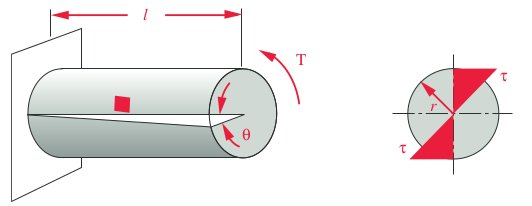
\includegraphics[width=\textwidth]{images/img501.jpg}
%	\end{center}
%	\fonte{**Norton 4ed**}
%\end{figure}
%
%\begin{equation}\label{eq:Eq_505}
%\theta = \frac{Tl}{GJ}
%\end{equation}
%
%\begin{equation}\label{eq:Eq_506}
%\tau = \frac{Tr}{J}
%\end{equation}
%
%\vspace{\baselineskip}
%
%\section{Sensoriamento de deformações}
%
%\subsection{Strain gauge}
%
%Strain gauges são sensores que sofrem alterações de resistência elétrica conforme a deformação ocorrida na superfície em que são aplicados, uma relação entre a variação de resistência e deformação em um strain gauge é denominado gauge factor.
%
%\begin{equation}\label{eq:Eq_507}
%K\varepsilon = \frac{\Delta R_{s}}{R_{s}}
%\end{equation}
%
%onde
%
%K: Gauge factor
%
%$\Delta R_{s}$: variação de resistência no strain gauge
%
%$R_{s}$: resistência nominal do strain gauge
%
%\vspace{\baselineskip}
%
%O resistor a ser utilizado é do modelo B350-3AA, que possui resistência nominal de 350 ohms e gauge factor de 2. 
%
%\subsection{Ponte de Wheatstone}
%
%Devido às pequenas variações de resistência durante o funcionamento do strain gauge, o que gera pequenas variações de tensão em seu funcionamento no circuito elétrico, é necessária sua montagem como parte de uma Ponte de Wheatstone. Esse tipo de montagem permite a instrumentação desses sensores, devido a melhor sensibilidade na leitura do voltímetro V.
%
%\begin{figure}[htb]
%	\caption{\label{fig:Fig_502}esquema basico de ponte de Wheatstone}
%	\begin{center}
%		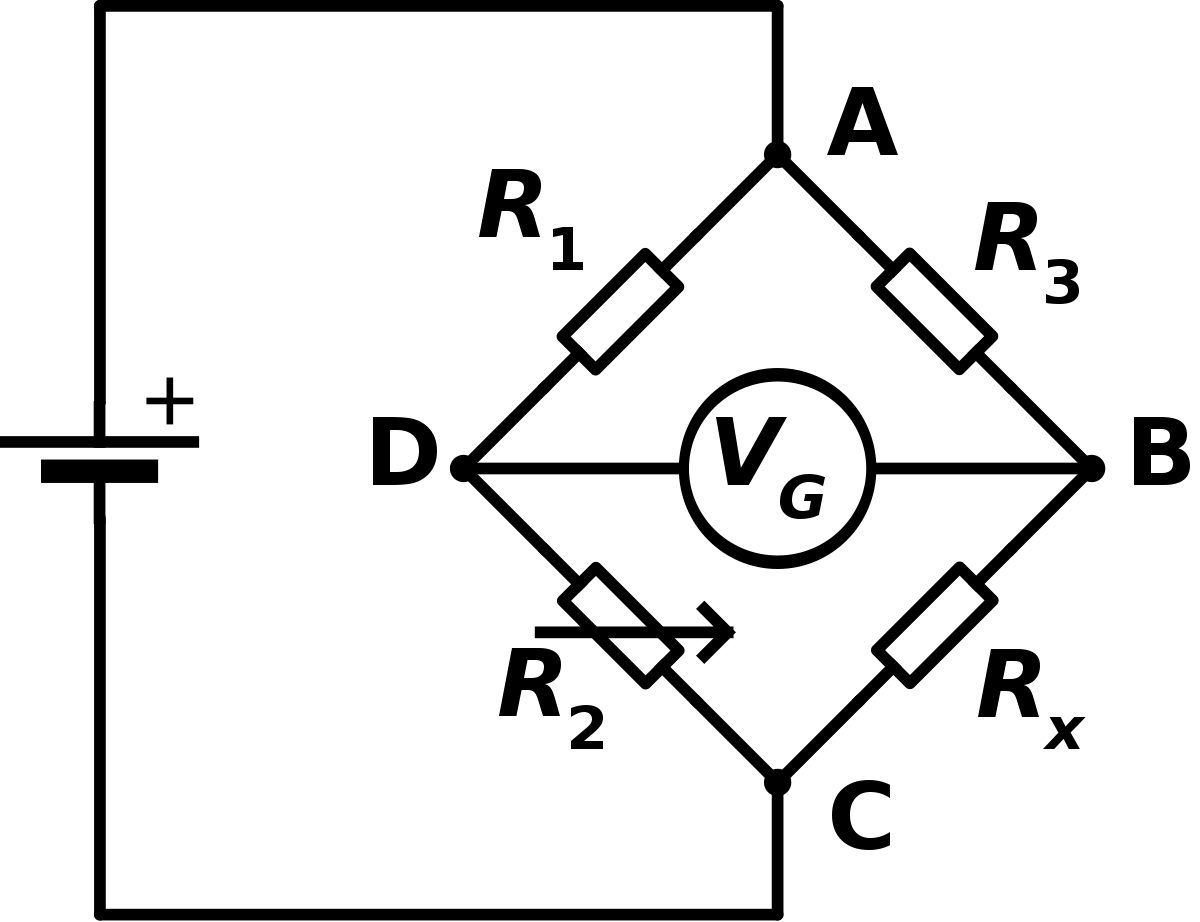
\includegraphics[width=\textwidth]{images/img502.png}
%	\end{center}
%	\fonte{*internet**}
%\end{figure}
%
%Substituindo a resistência R4 pelo strain gauge e utilizando resistores com resistências iguais ao do valor nominal do sensor em R1, R2 e R3, Utilizando as leis de Kirchoff para o circuito, a equação de transferência do circuito é encontrada.
%
%\begin{equation}\label{eq:Eq_508}
%\frac{V}{V_{in}} = \frac{K \varepsilon}{4 = K \varepsilon}
%\end{equation}
%
%onde
%
%Vin: Tensão de alimentação do circuito
%
%V: Tensão mostrada pelo voltímetro Vg



\chapter{Experimento}%\label{cap:Experimento}
%
%O presente capítulo demonstra a metodologia que será utilizada na execução do experimento e processamento dos dados obtidos.
%
%\vspace{\baselineskip}
%- Componentes necessários
%
%- Bancada Nat Geo
%
%- Comunicação Arduino PC
%
%- Pós processamento de dados
%
%- Pesquisas de metodologia de projeto
%
%- Projeto do dispositivo
%
%\section{Análise computacional}
%
%Descrever as rotinas computacionais desenvolvidas e seus resultados
%
%\vspace{\baselineskip}
%- Simulação feita no python
%
%- Resultados de torque esperados para aplicações
%
%- Verificar se os componentes são adequados
%
%\section{Microprocessador}
%
%Arduino (Documentação Arduino): “plataforma eletrônica de código aberto baseado em hardwares e softwares fáceis de usar” “as placas são capazes de ler entradas, e transformadas em saídas” “você pode dizer a sua placa o que fazer enviando um conjunto de informações ao microcontrolador na placa. Para isso, você utiliza a linguagem de programação Arduino, e o Arduino software (IDE), baseado em processamento” “Professores e estudantes utilizam para construção de instrumentos científicos de baixo custo. Designers e arquitetos constroem protótipos interativos” Vantagens: inexpensive, cross-platform, simple, clear programming environment, open source and extensible software and hardware
%
%Função analogRead(): Função que lê o valor relativo a tensão no pino de análise, sua saída varia entre 0 e 1023, o que significa 0 a 5V respectivamente (dependendo da placa pode ser 0 a 3.3V) (0.0049mV/unidade) “it takes around 100 microseconds (0.0001s) to read an analog input, so the maximum reading rate is about 10KHz”
%
%\section{Obtenção dos sinais}
%
%Análise no domínio do tempo de sistemas em tempo discreto (Lathi): “um sinal em tempo discreto é basicamente uma sequência de números. [...] podem aparecer como resultado da amostragem de sinais contínuos no tempo em sistemas amostrados de filtragem digital.”, “sistemas cujas entradas e saídas são sinais em tempo discreto são chamados de sistemas em tempo discreto ou simplesmente sistemas discretos. Um computador digital é um exemplo típico desse tipo de sistema. ”
%
%Amostragem: a ponte entre o contínuo e o discreto: “Um sinal em tempo contínuo pode ser processado, a partir de suas amostras, por um sistema que opere em tempo discreto. para isso, é importante manter a taxa de amostragem do sinal suficientemente alta para permitir a reconstrução sem erro (ou com um erro dentro de uma dada tolerância) do sinal original”, “O teorema da amostragem é a ponte entre os mundos de tempo contínuo e tempo discreto. A informação inerente em um sinal em tempo contínuo amostrado é equivalente a de um sinal em tempo discreto”
%
%Teorema da amostragem: Lathi demonstra que “um sinal em tempo real cujo espectro é limitado em faixa a B Hz pode ser reconstruído exatamente (sem qualquer erro) de suas amostras tomadas uniformemente a uma taxa de fz > 2B Hz”
%
%Conversão analógica para digital: “um sinal analógico é caracterizado pelo fato de sua amplitude poder assumir qualquer valor em um faixa contínua [...] um sinal analógico pode ser convertido em um sinal digital através de amostragem e quantização (arredondamento).”
%
%\vspace{\baselineskip}
%fig 8-14: conversão analógica pra digital (A/D)
%\vspace{\baselineskip}
%
%\section{Processamento dos dados}
%
%\section{Validação do dispositivo}
%
%-Calibração do dispositivo
%
%-Testes experimentais utilizando a bancada do nat geo
%
%*Falar sobre as ferramentas de validação estatística e seus resultados nas analises.



\phantomsection


\chapter{Resultados}%\label{cap:Resultados}


\phantomsection

\chapter{Conclusões}%\label{cap:Conclusões}
